\section{Chain Homotopies}


\begin{remark*}[Quotient categories]
  \label{quotient categories}
  Let~$\Ccat$ be a category and let~$\Acat$ be a preadditve category.
  \begin{enumerate}
    \item
      Suppose that we are given for any two objects~$X, Y \in \Ccat$ an equivalence relation~$\sim_{X,Y}$ of~$\Ccat(X,Y)$.
      Then we can try to define a \emph{quotient category}\index{quotient category}\index{category!quotient}~$\widetilde{\Ccat}$, that is supposed to be given by
      \begin{itemize}
        \item
          by the class of objects $\Ob(\widetilde{\Ccat}) \defined \Ob(\Ccat)$, and
        \item
          for any two objects~$X, Y \in \Ob(\widetilde{\Ccat}) = \Ob(\Ccat)$ the set of morphisms
          \[
                      \widetilde{\Ccat}(X,Y)
            \defined  \Ccat(X,Y)/{\sim_{X,Y}} \,,
          \]
        \item
          with the composition of~$[f] \in \widetilde{\Ccat}(X,Y)$ and~$g \in \widetilde{\Ccat}(Y,Z)$ being given by
          \[
                      [g] \circ [f]
            \defined  [g \circ f] \,.
          \]
      \end{itemize}
      However, the composition in~$\widetilde{\Ccat}$ will not be~{\welldef} in general.
      More specifically, this composition is~{\welldef} if and only if it holds for all morphisms~$f, f' \colon X \to Y$ and~$g, g' \colon Y \to Z$ in~$\Ccat$ that
      \begin{equation}
        \label{definition of congruence relation}
        \text{$f \sim_{X,Y} f'$ and~$g \sim_{Y,Z} g'$}
        \implies
        g \circ f \sim_{X,Z} g' \circ f' \,.
      \end{equation}
      If this condition is satisfied then~$\widetilde{\Ccat}$ is indeed a category:
      The associativity of compositions of morphisms is inherited from~$\Ccat$, and for every obect~$X \in \Ob(\widetilde{\Ccat}) = \Ob(\Ccat)$ the identity~$\id^{\widetilde{\Ccat}}_X$ is given by
      \[
          \id^{\widetilde{\Ccat}}_X
        = \left[ \id^{\Ccat}_X \right] \,.
      \]
      
      The collection of equivalence relations~$\sim \defined (\sim_{X,Y})_{X, Y \in \Ob(\Ccat)}$ is then a \emph{congruence relations}\index{congruence relation} on~$\Ccat$, and the quotient category~$\widetilde{\Ccat}$ as described above is denoted by~$\Ccat/{\sim}$.
      The equivalencen relations~$\sim_{X,Y}$ are for simplicity just denoted by~$\sim$.
      
      One may also think about a congruence relation on~$\Ccat$ as an equivalence relations on the class~$\coprod_{X, Y \in \Ob(\Ccat)} \Ccat(X,Y)$ of all morphisms in~$\Ccat$, that is compatible with domains, codomains and composition of morphisms.
      
      It is also worthwile to notice that the single condition~\eqref{definition of congruence relation} can equivalently be replaced by the two conditions
      \[
                  f \sim f'
        \implies  g \circ f \sim g \circ f'
      \]
      for all morphisms~$f, f' \colon X \to Y$ and~$g \colon Y \to Z$ in~$\Ccat$, and
      \[
                  f \sim f'
        \implies  f \circ h \sim f' \circ h
      \]
      for all morphisms~$f, f' \colon X \to Y$ and~$h \colon W \to X$ in~$\Ccat$.
    \item
      If~$\sim$ is a congruence relation on~$\Ccat$ then we get a \emph{projection functor}\index{projection functor}\index{functor!projection}
      \[
                P
        \colon  \Ccat
        \to     \Ccat/{\sim}
      \]
      that is given on objects by~$P(X) = X$ and on morphisms by~$P(f) = [f]$.
      This projection functor has the property that~$P(f) = P(f')$ for any two morphisms~$f$ and~$f'$ in~$\Ccat$ with~$f \sim f'$, and the functor~$P$ is universal with this property:
      Whenever~$F \colon \Ccat \to \Dcat$ is another functor such that~$F(f) = F(f')$ for all morphisms~$f$ and~$f'$ in~$\Ccat$ with~$f \sim f'$, then there exists a unique induced functor~$F' \colon (\Ccat/{\sim}) \to \Dcat$ that makes the following triangle commute:
      \[
        \begin{tikzcd}
            \Ccat
            \arrow{r}[above]{F}
            \arrow{d}[left]{P}
          & \Dcat
          \\
            \Ccat/{\sim}
            \arrow[dashed]{ur}[below right]{F'}
          & {}
        \end{tikzcd}
      \]
    \item
      Let~$\sim$ be a congruence relation on~$\Acat$.
      Then we would like the preadditive structure of~$\Acat$ to descend to a preadditive structure on~$\Acat/{\sim}$ via
      \[
                  [f] + [g]
        \defined  [f + g]
      \]
      for any two parallel morphisms~$[f], [g] \colon X \to Y$ in~$\Acat/{\sim}$.
      This addition of morphisms in the quotient category~$\Acat/{\sim}$ is {\welldef} if and only if it holds for all morphisms~$f, f', g, g' \colon X \to Y$ in~$\Acat$ that
      \[
        \text{$f \sim f'$ and~$g \sim g'$}
        \implies
        f + g \sim f' + g' \,.
      \]
      The congruence relation~$\sim$ is then called \emph{additive}\index{additive!congruence relation}\index{congruence relation!additive}.
      
      If~$\sim$ is additive then~$\Acat/{\sim}$ is together with the above addition of morphisms indeed a preadditive category:
      The associativity of the addition on~$(\Acat/{\sim})(X,Y)$ is inherited from~$\Acat(X,Y)$.
      The neutral element of~$(\Acat/{\sim})(X,Y)$ is given by the morphism~$[0]$, and the additive inverse of a morphism~$[f] \in (\Acat/{\sim})(X,Y)$ is given by the morphism~$[-f]$.
      The bilinearity of the composition of morphisms in~$\Acat/{\sim}$ follows from the bilinearity of the composition of morphisms in~$\Acat$.
      
      Note that if~$\sim$ is additive then the projection functor~$P \colon \Acat \to \Acat/{\sim}$ is additive.
    \item
      An \emph{ideal}~$\Ideal$\index{ideal} in~$\Acat$ consists of a subgroup~$\Ideal(X,Y) \subseteq \Acat(X,Y)$ for any two objects~$X, Y \in \Ob(\Acat)$ such that
      \[
                  \Acat(Y,Z) \circ \Ideal(X,Y)
        \subseteq \Ideal(X,Z)
        \quad\text{and}\quad
                  \Ideal(X,Y) \circ \Acat(W,X)
        \subseteq \Ideal(W,Y)
      \]
      for all objects~$W, X, Y, Z \in \Ob(\Acat)$.
    \item
      Additive congruence relations on~$\Acat$ are in {\onetoone} correspondence with ideals in~$\Acat$:
      
      If~$F \colon \Acat \to \Bcat$ is any additive functor, where~$\Bcat$ is another preadditive category, then
      \begin{align*}
                  \ker(F)(X,Y)
        &\defined \{
                    f \in \Acat(X,Y)
                  \suchthat
                    F(f) = 0
                  \}  \\
        &=        \ker\Bigl( \Acat(X,Y) \xlongto{F} \Bcat(F(X),F(Y)) \Bigr)
      \end{align*}
      is for any two objects~$X, Y \in \Ob(\Acat)$ a subgroup of~$\Acat(X,Y)$.
      This collection of subgroups defines an ideal~$\ker(F)$ in~$\Acat$, the \emph{kernel}\index{kernel!of an additive functor}\index{functor!additive!kernel}\index{additive!functor!kernel} of~$F$
      If~$\sim$ is an additive congruence relation on~$\Acat$ then the projection functor~$P \colon \Acat \to (\Acat/{\sim})$ is additive, and hence~$\Ideal \defined \ker(P)$ is an ideal in~$\Acat$.
      This ideal~$\Ideal$ in~$\Acat$ is given by
      \[
          \Ideal(X,Y)
        = \{
              f \in \Acat(X,Y)
            \suchthat
              P(f) = 0
            \}
        =   \{
              f \in \Acat(X,Y)
            \suchthat
              f \sim 0
            \}
      \]
      for all~$X, Y \in \Ob(\Acat)$.
      
      If on the other hand~$\Ideal$ is an ideal in~$\Acat$ then we can define an additive congruence relation~$\sim$ on~$\Acat$ that is given by
      \[
              f \sim g
        \iff  f - g \in \Ideal(X,Y)
      \]
      for any two parallel morphisms~$f, g \colon X \to Y$ in~$\Acat$.
      Indeed, it is known from basic algebra that~$\sim$ defines for all~$X, Y \in \Ob(\Acat)$ an equivalence relation on~$\Acat(X,Y)$ that is compatible with the addition on~$\Acat(X,Y)$, in the sense that
      \[
        \text{$f \sim f'$ and~$g \sim g'$}
        \implies
        f + g \sim f' + g'
      \]
      for all morphisms~$f, f', g, g' \in \Acat(X,Y)$.
      (This equivalence relation on~$\Acat(X,Y)$ is the one used to construct the quotient group~$\Acat(X,Y)/\Ideal(X,Y)$.)
      If~$f, f' \colon X \to Y$ and~$g, g' \colon Y \to Z$ are morphisms in~$\Acat$ with~$f \sim f'$ and~$g \sim g'$ then
      \[
            gf - g'f'
        =   gf - gf' + gf' - g'f'
        =   g(f - f') + (g - g')f'
        \in \Ideal(X,Z)
      \]
      because~$f - f' \in \Ideal(X,Y)$ and~$g - g' \in \Ideal(Y,Z)$ and because~$\Ideal$ is an ideal.
      Hence also~$gf \sim g' f'$.
      This shows altogether that~$\sim$ is indeed an additive congruence relation on~$\Acat$.
      
      These two constructions are mutually inverse, and give a {\onetoone} correspondence between additive congruence relations in~$\Acat$ and ideals in~$\Acat$.
      
      If~$\Ideal$ is an ideal in~$\Acat$ with corresponding additive congruence relation~$\sim$ then we define the quotient of~$\Acat$ by~$\Ideal$ as
      \[
                  \Acat/\Ideal
        \defined  \Acat/{\sim} \,.
      \]
      This is by the above discussion again a preadditive category, and we have that the projection functor~$\Acat \to \Acat/\Ideal$ is additive (by construction of the preadditive structure on~$\Acat/\Ideal$).
      We note that the morphisms groups of~$\Acat/\Ideal$ are for any two objects~$X, Y \in \Ob(\Acat/\Ideal) = \Ob(\Acat)$ given by
      \[
          (\Acat/\Ideal)(X,Y)
        = \Acat(X,Y)/\Ideal(X,Y) \,.
      \]
    \item
      If~$\Ideal$ and~$\Jdeal$ are two ideal in~$\Acat$ then the ideal~$\Ideal$ is a \emph{subideal}\index{subideal} of the ideal~$\Jdeal$, denoted by~$\Ideal \subseteq \Jdeal$, if~$\Ideal(X,Y) \subseteq \Jdeal(X,Y)$ for all~$X, Y \in \Ob(\Acat)$.
      
      If~$\Ideal$ is an ideal in~$\Acat$ with corresponding additive equivalence relation~$\sim$ on~$\Acat$, then the aforementioned universal propery of the quotient category~$\Acat/{\sim}$ leads to the following universal property of the quotient category~$\Acat/\Ideal$:
      If~$F \colon \Acat \to \Bcat$ is an additive functor, where~$\Bcat$ is another preadditive category, then~$F$ decends to a functor~$F' \colon \Acat/\Ideal \to \Bcat$ that makes the triangle
      \[
        \begin{tikzcd}
            \Acat
            \arrow{r}[above]{F}
            \arrow{d}[left]{P}
          & \Bcat
          \\
            \Acat/\Ideal
            \arrow[dashed]{ur}[below right]{F'}
          & {}
        \end{tikzcd}
      \]
      commute if and only if~$\Ideal \subseteq \ker(F)$.
      The induced functor~$F'$ is then unique with this property and again additive.
    \item
      If~$\Acat$ is an additive category and~$\Ideal$ is an ideal in~$\Acat$ then the resulting quotient category~$\Acat/\Ideal$ is again additive:
      Let~$X_1, \dotsc, X_n$ be finitely many objects in~$\Ob(\Acat/\Ideal)$ and let~$(X, (c_i)_{i=1}^n, (p_i)_{i=1}^n)$ be a biprodct of~$X_1, \dotsc, X_n$ in~$\Acat$.
      Then~$(X, ([c_i])_{i=1}^n, ([p_i])_{i=1}^n)$ is a biproduct of~$X_1, \dotsc, X_n$ in~$\Acat/\Ideal$ because the projection functor~$P \colon \Acat \to \Acat/\Ideal$ respects biproducts by part~\ref{additive preserves biproducts} of \cref{characterizations of additive functors}.
  \end{enumerate}
\end{remark*}


\begin{example*}
  \leavevmode
  \begin{enumerate}
    \item
      In the category~$\Top$ of topological spaces a congruence relation~$\sim$ is given by
      \[
              f \sim g
        \iff  \text{$f$ and~$g$ are homotopic}
      \]
      for any two parallel continuous maps~$f, g \colon X \to Y$.
      The resulting quotient category~$\Top/{\sim}$ is precisely the homotopy category~$\hTop$.
    \item
      We may regard a ring~$R$ as a preadditive category~$\Rcat$ that consists of a single object~$\ast$, for which~$\Rcat(\ast, \ast) = R$.
      Then an ideal~$\Ideal$ in the category~$\Rcat$ is the same as an additive subgroup~$I = \Ideal(X,X)$ of~$R$ that satisfies~$RI = I$ and~$IR = R$.
      In other words, ideals in~$\Rcat$ are the same as {\twosided} ideals in~$R$.
      
      We also note that the quotient category~$\Rcat/\Ideal$ is then precisely the quotient ring~$R/I$ regarded as a \dash{one}{object} preadditive category.
    \item
      If~$G$ is a group, then we can similarly regard~$G$ as a category~$\Gcat$ consisting of a single object~$\ast$ for which~$\Gcat(\ast,\ast) = G$.
      Then a congruence relations~$\sim$ in~$\Gcat$ is the same as normal subgroup~$N$ of~$G$ via
      \[
                  N
        \defined  \{
                    g \in G
                  \suchthat
                    g \sim 1
                  \} \,.
      \]
      The quotient category~$\Gcat/{\sim}$ is then precisely the quotient group~$G/N$ regarded as a \dash{single}{object} category.
  \end{enumerate}
\end{example*}


\begin{warning*}
  If~$\Acat$ is an abelian category and~$\Ideal$ is an ideal in~$\Acat$ then the quotient category~$\Acat/\Ideal$, which is again additive, won’t necessarily be abelian again.
\end{warning*}


\begin{definition}
  \leavevmode
  \begin{enumerate}
    \item 
      Let~$\Ccc$ and~$\Dcc$ be two chain complexes in~$\Acat$, and let~$f, g \colon \Ccc \to \Dcc$ be two parallel morphisms of chain complexes.
      \begin{enumerate}
        \item
          The morphism~$f = (f_n)_{n \in \Integer}$ is \emph{null homotopic}\index{null!homotopic} if there exists a family~$(s_n)_{n \in \Integer}$ of morphisms~$s_n \colon C_n \to D_{n+1}$ such that~$f = ds + sd$, i.e.\ such that
          \[
                f_n
            =  d_{n+1} s_n + s_{n-1} d_n
          \]
            for every~$n \in \Integer$.
        \item
          The morphisms~$f$ and~$g$ are \emph{homotopic}\index{homotopic} if their difference~$f - g$ is null homotopic.
          That the morphisms~$f$ and~$g$ are homotopic is denoted by~$f \sim g$.
        \item
          The morphism~$f$ is a \emph{homotopy equivalence}\index{homotopy!equivalence} if there exist a morphism of chain complexes~$h \colon \Dcc \to \Ccc$ such that~$f h \sim \id_{\Dcc}$ and~$h f \sim \id_{\Ccc}$.
      \end{enumerate}
    \item
      Let~$\Cccc$ and~$\Dccc$ be two cochain complexes in~$\Acat$, and let~$f, g \colon \Cccc \to \Dccc$ be two parallel morphisms of cochain complexes.
      \begin{enumerate}
        \item
          The morphism~$f = (f^n)_{n \in \Integer}$ is \emph{null homotopic}\index{null!homotopic} if there exists a family~$(s^n)_{n \in \Integer}$ of morphisms~$s^n \colon C^n \to D^{n-1}$ such that~$f = ds + sd$, i.e.\ such that
          \[
              f^n
            = d^{n-1} s^n + s^{n+1} d^n
          \]
          for every~$n \in \Integer$.
        \item
          The morphisms~$f$ and~$g$ are \emph{homotopic}\index{homotopic} if their difference~$f - g$ is null homotopic.
          That the morphisms~$f$ and~$g$ are homotopic is denoted by~$f \sim g$.
        \item
          The morphisms~$f$ is a \emph{homotopy equivalence}\index{homotopy!equivalence} if there exist a morphism of cochain complexes~$h \colon \Dccc \to \Cccc$ such that~$f h \sim \id_{\Dccc}$ and~$h f \sim \id_{\Cccc}$.
      \end{enumerate}
  \end{enumerate}
\end{definition}


\begin{remark*}
  Let~$\Ccc$ and~$\Dcc$ be two chain complexes in~$\Acat$ and let~$f, g \colon \Ccc \to \Dcc$ be two parallel morphisms of chain complexes.
  \begin{enumerate}
    \item
      A family~$s = (s_n)_{n \in \Integer}$ of morphisms~$s_n \colon C_n \to D_{n+1}$ with~$f = ds + sd$ is a \emph{null homotopy}\index{null!homotopy}\index{homotopy!null} for~$f$.
      Such a null homotopy~$s$ for~$f$ may be visualized as the diagram
      \[
        \begin{tikzcd}[column sep =  large, row sep = huge]
            \dotsb
            \arrow{r}
          & C_{n+1}
            \arrow{r}[above]{d_{n+1}}
            \arrow{d}[right, near start]{f_{n+1}}
            \arrow[dashed]{dl}
          & C_n
            \arrow{r}[above]{d_n}
            \arrow{d}[right, near start]{f_n}
            \arrow[dashed]{dl}[below right]{s_n}
          & C_{n-1}
            \arrow{r}
            \arrow{d}[right, near start]{f_{n-1}}
            \arrow[dashed]{dl}[below right]{s_{n-1}}
          & \dotsb
            \arrow[dashed]{dl}
          \\
            \dotsb
            \arrow{r}
          & D_{n+1}
            \arrow{r}[above]{d_{n+1}}
          & D_n
            \arrow{r}[above]{d_n}
          & D_{n-1}
            \arrow{r}
          & \dotsb
        \end{tikzcd}
      \]
      together with the formula
      \[
          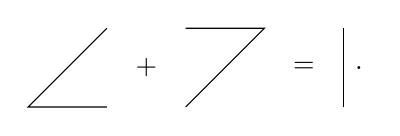
\begin{tikzpicture}
            \draw (1,1) -- (0,0)-- (1,0);
            \draw (1.5,0.5) node{$+$};
            \draw (2,1) -- (3,1) -- (2,0);
            \draw (3.5,0.5) node{$=$};
            \draw (4,1) -- (4,0);
            \draw (4.2,0.5) node {.};
          \end{tikzpicture}
      \]
    \item
      A family~$s = (s_n)_{n \in \Integer}$ of morphisms~$s_n \colon C_n \to D_{n+1}$ with~$f-g = ds + sd$, i.e.\ a null homotopy for~$f-g$, is a \emph{homotopy}\index{homotopy} between~$f$ and~$g$.
  \end{enumerate}
\end{remark*}


\begin{remark}
  Let~$\Ccc$ and~$\Dcc$ be morphisms of chain complexes in~$\Acat$.
  If~$(s_n)_{n \in \Natural}$ is any family of morphisms~$s_n \colon C_n \to D_{n+1}$ then~$f \defined (f_n)_{n \in \Integer}$ with~$f_n \defined d_{n+1} s_n + s_{n-1} d_n$ is a morphism of chain complexes~$f \colon \Ccc \to \Dcc$ because
  \[
      d{}f
    = d (ds + sd)
    = d^2 s + dsd
    = dsd
    = dsd + sd^2
    = (ds + sd) d
    = f d \,.
  \]
\end{remark}

\begin{lemma}
  Let~$\Ccc$ and~$\Dcc$ be chain complexes and let~$f, g \colon \Ccc \to \Dcc$ be two parallel morphisms.
  \begin{enumerate}
    \item
      \label{null homotopic is zero in homotopy}
      If the morphism~$f$ is null homotopic then~$\Hl_n(f) = 0$ for every~$n \in \Integer$.
    \item
      \label{homotopic morphisms are the same in homotopy}
      If the morphisms~$f$ and~$g$ are homotopic then~$\Hl_n(f) = \Hl_n(g)$ for every~$n \in \Integer$.
    \item
      If~$f$ is a homotopy equivalence then~$f$ is a {\qim}.
  \end{enumerate}
  The same holds for cochain complexes.
\end{lemma}


\begin{proof}
  \leavevmode
  \begin{enumerate}
    \item
      This is Exercise~1 of Exercise~sheet~9.
    \item
      This follows from part~\ref*{null homotopic is zero in homotopy} by the additivity of~$\Hl_n$.
    \item
      This follows from part~\ref*{homotopic morphisms are the same in homotopy} by the functoriality of~$\Hl_n$.
    \qedhere
  \end{enumerate}
\end{proof}


\begin{remark}
  At this point in the lecture it was remarked that the homology functors~$\Hl_n \colon \Ch(\Acat) \to \Acat$ are additive.
  We have (thanks to some personal modifications) already seen this (in a slightly different way than in the lecture) in~\cref{functoriality of homology}.
%   We have seen in~\cref{functoriality of homology} that the functors~$\Hl_n \colon \Ch(\Acat) \to \Acat$ with~$n \in \Integer$ are additive, but this can also seen as follows:
%   
%   For any two morphisms~$f_1 \colon X_1 \to Y_1$ and~$f'_2 \colon X_2 \to Y_2$ in~$\Acat$, then we get the combined morphism
%   \[
%             \begin{bmatrix}
%               f_1 &     \\
%                   & f_2
%             \end{bmatrix}
%     \colon  X_1 \oplus X_2
%     \to     Y_1 \oplus Y_2 \,.
%   \]
%   If~$k_1 \colon \ker(f_1) \to X_1$ is a kernel of~$f_1$ and~$k_2 \colon \ker(f_2) \to X_2$ is a kernel of~$f_2$, then
%   \[
%             \begin{bmatrix}
%               k_1 &     \\
%                   & k_2
%             \end{bmatrix}
%     \colon  \ker(f_1) \oplus \ker(f_2)
%     \to     X_1 \oplus X_2
%   \]
%   is a kernel of~$\begin{bsmallmatrix} f_1 & \\ & f_2 \end{bsmallmatrix}$.
%   Dually, if~$c_1 \colon Y_1 \to \coker(f_1)$ and~$c_2 \colon Y_2 \to \coker(f_2)$ are cokernels of~$f_1$ and~$f_2$ then
%    \[
%             \begin{bmatrix}
%               c_1 &     \\
%                   & c_2
%             \end{bmatrix}
%     \colon  Y_1 \oplus Y_2
%     \to     \coker(f_1) \oplus \coker(f_2)
%   \]
%   is a cokernel of~$\begin{bsmallmatrix} f_1 & \\ & f_2 \end{bsmallmatrix}$.
%   It also follows by combining both of these observations that if~$i_1 \colon \im(f_1) \to Y_1$ and~$i_2 \colon \im(f_2) \to Y_2$ are images of~$f_1$ and~$f_2$, then
%   \[
%             \begin{bmatrix}
%               i_1 &     \\
%                   & i_2
%             \end{bmatrix}
%     \colon  \im(f_1) \oplus \im(f_2)
%     \to     Y_1 \oplus Y_2
%   \]
%   is a cokernel of~$\begin{bsmallmatrix} f_1 & \\ & f_2 \end{bsmallmatrix}$.
%   
%   Let~$\Ccc^{(1)}$ and~$\Ccc^{(2)}$ be two chain complexes.
%   For~$j = 1, 2$ let
%   \[
%     p^{(j)}_n \colon C^{(j)}_{n-1} \to \Bl_n(\Ccc^{(j)})
%     \quad\text{and}\quad
%     i^{(j)}_n \colon \Zl_n(\Ccc^{(j)}) \to C^{(j)}_n
%   \]
%   be the canonical morphisms and let~$\lambda^{(j)} \colon \Bl_n(\Ccc^{(j)}) \to \Zl_n(\Ccc^{(j)})$ be the canonical morphism, i.e.\ the unique morphism that makes the following diagram commute:
%   \[
%     \begin{tikzcd}[column sep = tiny]
%         \dotsb
%         \arrow{rr}
%       & {}
%       & C^{(j)}_{n+1}
%         \arrow{rr}[above]{d^{(j)}_{n+1}}
%         \arrow{dr}
%       & {}
%       & C^{(j)}_n
%         \arrow{rr}[above]{d^{(j)}_n}
%       & {}
%       & C^{(j)}_{n-1}
%         \arrow{rr}
%       & {}
%       & \dotsb
%       \\
%         {}
%       & {}
%       & {}
%       & \Bl_n(\Ccc^{(j)})
%         \arrow{ur}
%         \arrow[dashed]{rr}
%       & {}
%       & \Zl_n(\Ccc^{(j)})
%         \arrow{ul}
%       & {}
%       & {}
%       & {}
%     \end{tikzcd}
%   \]
%   The differential~$d$ of~$\Ccc^{(1)} \oplus \Ccc^{(2)}$ is given by
%   \[
%       d_n
%     = \begin{bmatrix}
%         d^{(1)}_n &           \\
%                   & d^{(2)}_n
%       \end{bmatrix}
%   \]
%   for every~$n \in \Integer$.
%   It follows from the above observations that
%   \[
%       \Zl_n( \Ccc^{(1)} \oplus \Ccc^{(2)} )
%     = \Zl_n(\Ccc^{(1)}) \oplus \Zl_n(\Ccc^{(2)}) \,,,
%   \]
\end{remark}


\begin{example}
  Let~$f, g \colon X \to Y$ be two continuous maps between topological spaces~$X$ and~$Y$.
  If the maps~$f$ and~$g$ are homotopic then their induced morphisms of chain complexes~$f_*, g_* \colon \Ccc^\sing(X) \to \Ccc^\sing(Y)$ are again homotopic.
\end{example}


\begin{remarkdefinition}
  \label{definition of homotopy category}
  Let~$\Bcc$,~$\Ccc$,~$\Dcc$ and~$\Ecc$ be chain complexes in~$\Acat$.
  \begin{enumerate}
    \item
      The set
      \[
          N
        = \{
            f \in \Hom_{\Ch(\Acat)}(\Ccc, \Dcc)
          \suchthat
            \text{$f$ is null homotopic}
          \}
      \]
      is a subgroup of~$\Hom_{\Ch(\Acat)}(\Ccc, \Dcc)$:
      \begin{itemize}
        \item
          It holds that~$0 \in \Hom_{\Ch(\Acat)}(\Ccc, \Dcc)$, i.e.\ the zero morphism is null homotopic.
          This can be seen by choosing for the required nullhomotpy~$s = (s_n)_{n \in \Integer}$ the zero morphism~$s_n = 0$ for every~$n \in \Integer$.
        \item
          If two morphisms of chain complexes~$f, g \colon \Ccc \to \Dcc$ are null homotopic then there exist null homotopies~$s = (s_n)_{n \in \Integer}$ and~$t = (t_n)_{n \in \Integer}$ for~$f$ and~$g$.
          Then~$u = (u_n)_{n \in \Integer}$ with~$u_n \defined s_n - t_n$ is a null homotopy for~$f - g$ because
          \begin{align*}
                du + ud
             =  d(s - t) + (s - t)d
            &=  ds - dt + sd - td \\
            &=  ds + sd - (dt + td)
             =  f - g \,.
          \end{align*}
          This show that for all~$f, g \in N$ also~$f - g \in N$.
      \end{itemize}
      It follows that homotopy of morphisms of chain complexes is an equivalence relation on~$\Hom_{\Ch(\Acat)}(\Ccc, \Dcc)$.
    \item
      \label{welldefinedness of sum}
      If~$f, f', g, g' \colon \Ccc \to \Dcc$ are morphisms of chain complexes with both~$f \sim g$ and~$f' \sim g'$ then also~$f + g \sim f' + g'$:
      We find for~$N$ as above that it follows from~$f - f', g - g' \in N$ that also
      \[
            (f + g) - (f' + g')
        =   (f - f') + (g - g')
        \in N \,,
      \]
      because~$N$ is a subgroup of~$\Hom_{\Ch(\Acat)}(X,Y)$.
    \item
      Let~$f \colon \Ccc \to \Dcc$ be a morphism of chain complexes that is null homotopic, say via a null homotopy~$(s_n)_{n \in \Integer}$.
      Then for every morphism of chain complexes~$g \colon \Dcc \to \Ecc$ the composition~$gf$ is again null homotopic:
      The family~$t = (t_n)_{n \in \Integer}$ given by~$t_n \defined g_{n+1} s_n$ is a null homotopy for~$gf$ because
      \[
          gf
        = g(ds + sd)
        = gds + gsd
        = dgs + gsd
        = dt + td \,.
      \]
      We find similarly that for every morphism of chain complexes~$h \colon \Bcc \to \Ccc$ the composition~$fh$ is again null homotopic:
      The family~$u = (u_n)_{n \in \Integer}$ given by~$u_n \defined s_n h_n$ is a null homotopy for~$fh$ because
      \[
          fh
        = (ds + sd)h
        = dsh + sdh
        = dsh + shd
        = du + ud \,.
      \]
      It follows for all morphisms of chain complexes~$f, f' \colon \Ccc \to \Dcc$ and~$g, g' \colon \Dcc \to \Ecc$ with~$f \sim f'$ and~$g \sim g'$ that also~$gf \sim g'f'$.
      Indeed, the difference
      \[
          gf - g'f'
        = gf - gf' + gf' - g'f'
        = g(f - f') + (g - g')f'
      \]
      is nullhomotpic because both~$f-f'$ and~$g-g'$ are null homotopic.
    \item
      This shows that the composition of morphisms in~$\Ch(\Acat)$ descends to a composition of equivalence classes with respect to homotopy.
      We hence obtain a category~$\Homotopy(\Acat)$ with
      \begin{itemize}
        \item
          objects~$\Ob(\Homotopy(\Acat)) \defined \Ob(\Ch(\Acat))$,
        \item
          morphism sets
          \begin{align*}
                        \Homotopy(\Acat)(\Ccc, \Dcc)
            \defined&{} \Hom_{\Ch(\Acat)}(\Ccc,\Dcc)/{\sim} \\
                   =&{} \Hom_{\Ch(\Acat)}(\Ccc,\Dcc)/\text{homotopy}
          \end{align*}
          for every two chain complexes~$\Ccc$ and~$\Dcc$ in~$\Acat$,
        \item
          and composition of morphisms~$[f] \colon \Ccc \to \Dcc$ and~$[g] \colon \Dcc \to \Ecc$ given by
          \[
                      [g] \circ [f]
            \defined  [g \circ f] \,.
          \]
      \end{itemize}
      The category~$\Homotopy(\Acat)$ is the \emph{homotopy category}\index{homotopy!category} of~$\Acat$.
    \item
      The homotopy category~$\Homotopy(\Acat)$ is again additve:
      The preadditive structure of~$\Homotopy(\Acat)$ is inherited from the category~$\Ch(\Acat)$ via
      \[
                  [f] + [g]
        \defined  [f + g]
      \]
      for any two parallel morphisms~$[f], [g] \colon \Ccc \to \Dcc$ in~$\Homotopy(\Acat)$.
      Part~\ref{welldefinedness of sum} shows that this addition is {\welldef}, and that~$\Homotopy(\Acat)$ satisfies the axioms of a preadditive category follows from~$\Ch(\Acat)$ satisfying these axioms.
      
      If~$\Ccc^{(1)}, \dotsc, \Ccc^{(n)}$ are finitely many chain complexes in~$\Acat$, i.e.\ objects of the homotopy category~$\Homotopy(\Acat)$, then a biproduct of~$\Ccc^{(1)}, \dotsc, \Ccc^{(n)}$ in~$\Homotopy(\Acat)$ is given by~$(\Ccc, ([c_i])_{i=1}^n, ([p_i])_{i=1}^n)$ if~$(\Ccc, (c_i)_{i=1}^n, (p_i)_{i=1}^n)$ is a biproduct of~$\Ccc^{(1)}, \dotsc, \Ccc^{(n)}$ in~$\Ch(\Acat)$.
  \end{enumerate}
\end{remarkdefinition}


\begin{warningnonum}
  Even though~$\Acat$ and~$\Ch(\Acat)$ are abelian, the homotopy category~$\Homotopy(\Acat)$ will in general not be abelian again.
  (A counterexample can be found in Exercise~4 of Exercise~sheet~9, where is shown that~$\Homotopy(\Ab)$ is not abelian.)
\end{warningnonum}


\begin{remark*}
  We may reformulate \cref{definition of homotopy category} using the language introduced in \cref{quotient categories}:
  The null homotopic morphisms of chain complexes form an ideal~$\Ndeal$ in the additive category~$\Ch(\Acat)$, whose corresponding additive congruence relation~$\sim$ is given by homotopy of morphisms of chain complex.
  The homotopy category~$\Homotopy(\Acat)$ is precisely the quotient category~$\Ch(\Acat)/\Ndeal = \Ch(\Acat)/{\sim}$.
\end{remark*}




